%% LyX 2.3.2 created this file.  For more info, see http://www.lyx.org/.
%% Do not edit unless you really know what you are doing.
\documentclass[english]{article}
\usepackage{mathpazo}
\usepackage[T1]{fontenc}
\usepackage[latin9]{inputenc}
\usepackage[letterpaper]{geometry}
\geometry{verbose,tmargin=1in,bmargin=1in,lmargin=1in,rmargin=1in}
\usepackage{graphicx}

\makeatletter
\@ifundefined{showcaptionsetup}{}{%
 \PassOptionsToPackage{caption=false}{subfig}}
\usepackage{subfig}
\makeatother

\usepackage{babel}
\begin{document}
\begin{figure}
\begin{centering}
\subfloat[a]{\begin{centering}
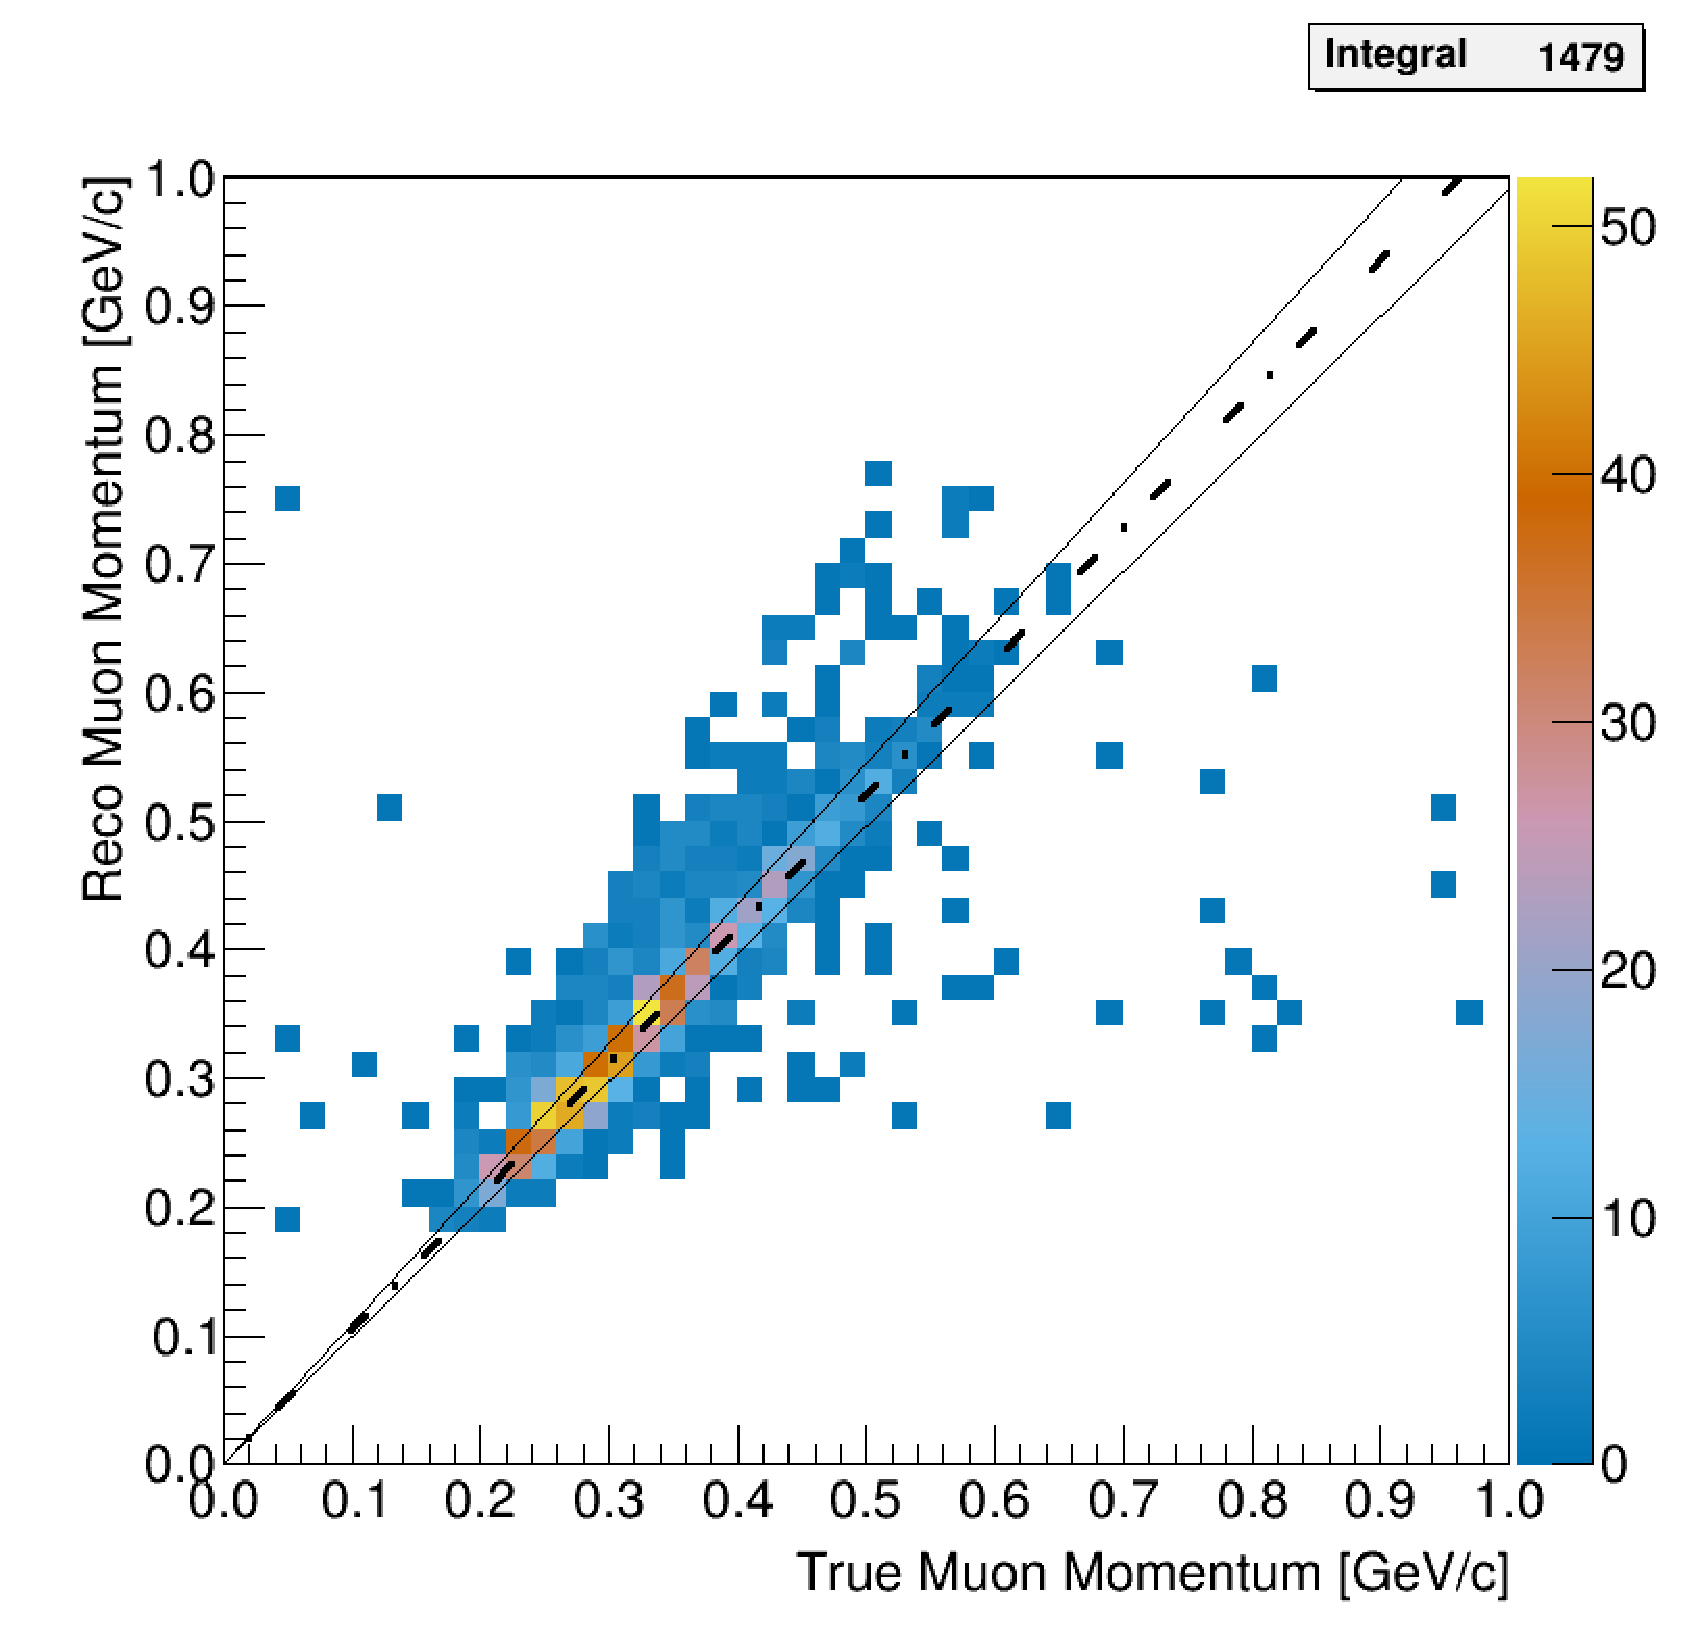
\includegraphics[width=0.48\textwidth]{Figures/P0DCC1pi/Contained_SignalMuons_UnCalib_reco_vs_true_p}
\par\end{centering}

}\subfloat[b]{\begin{centering}
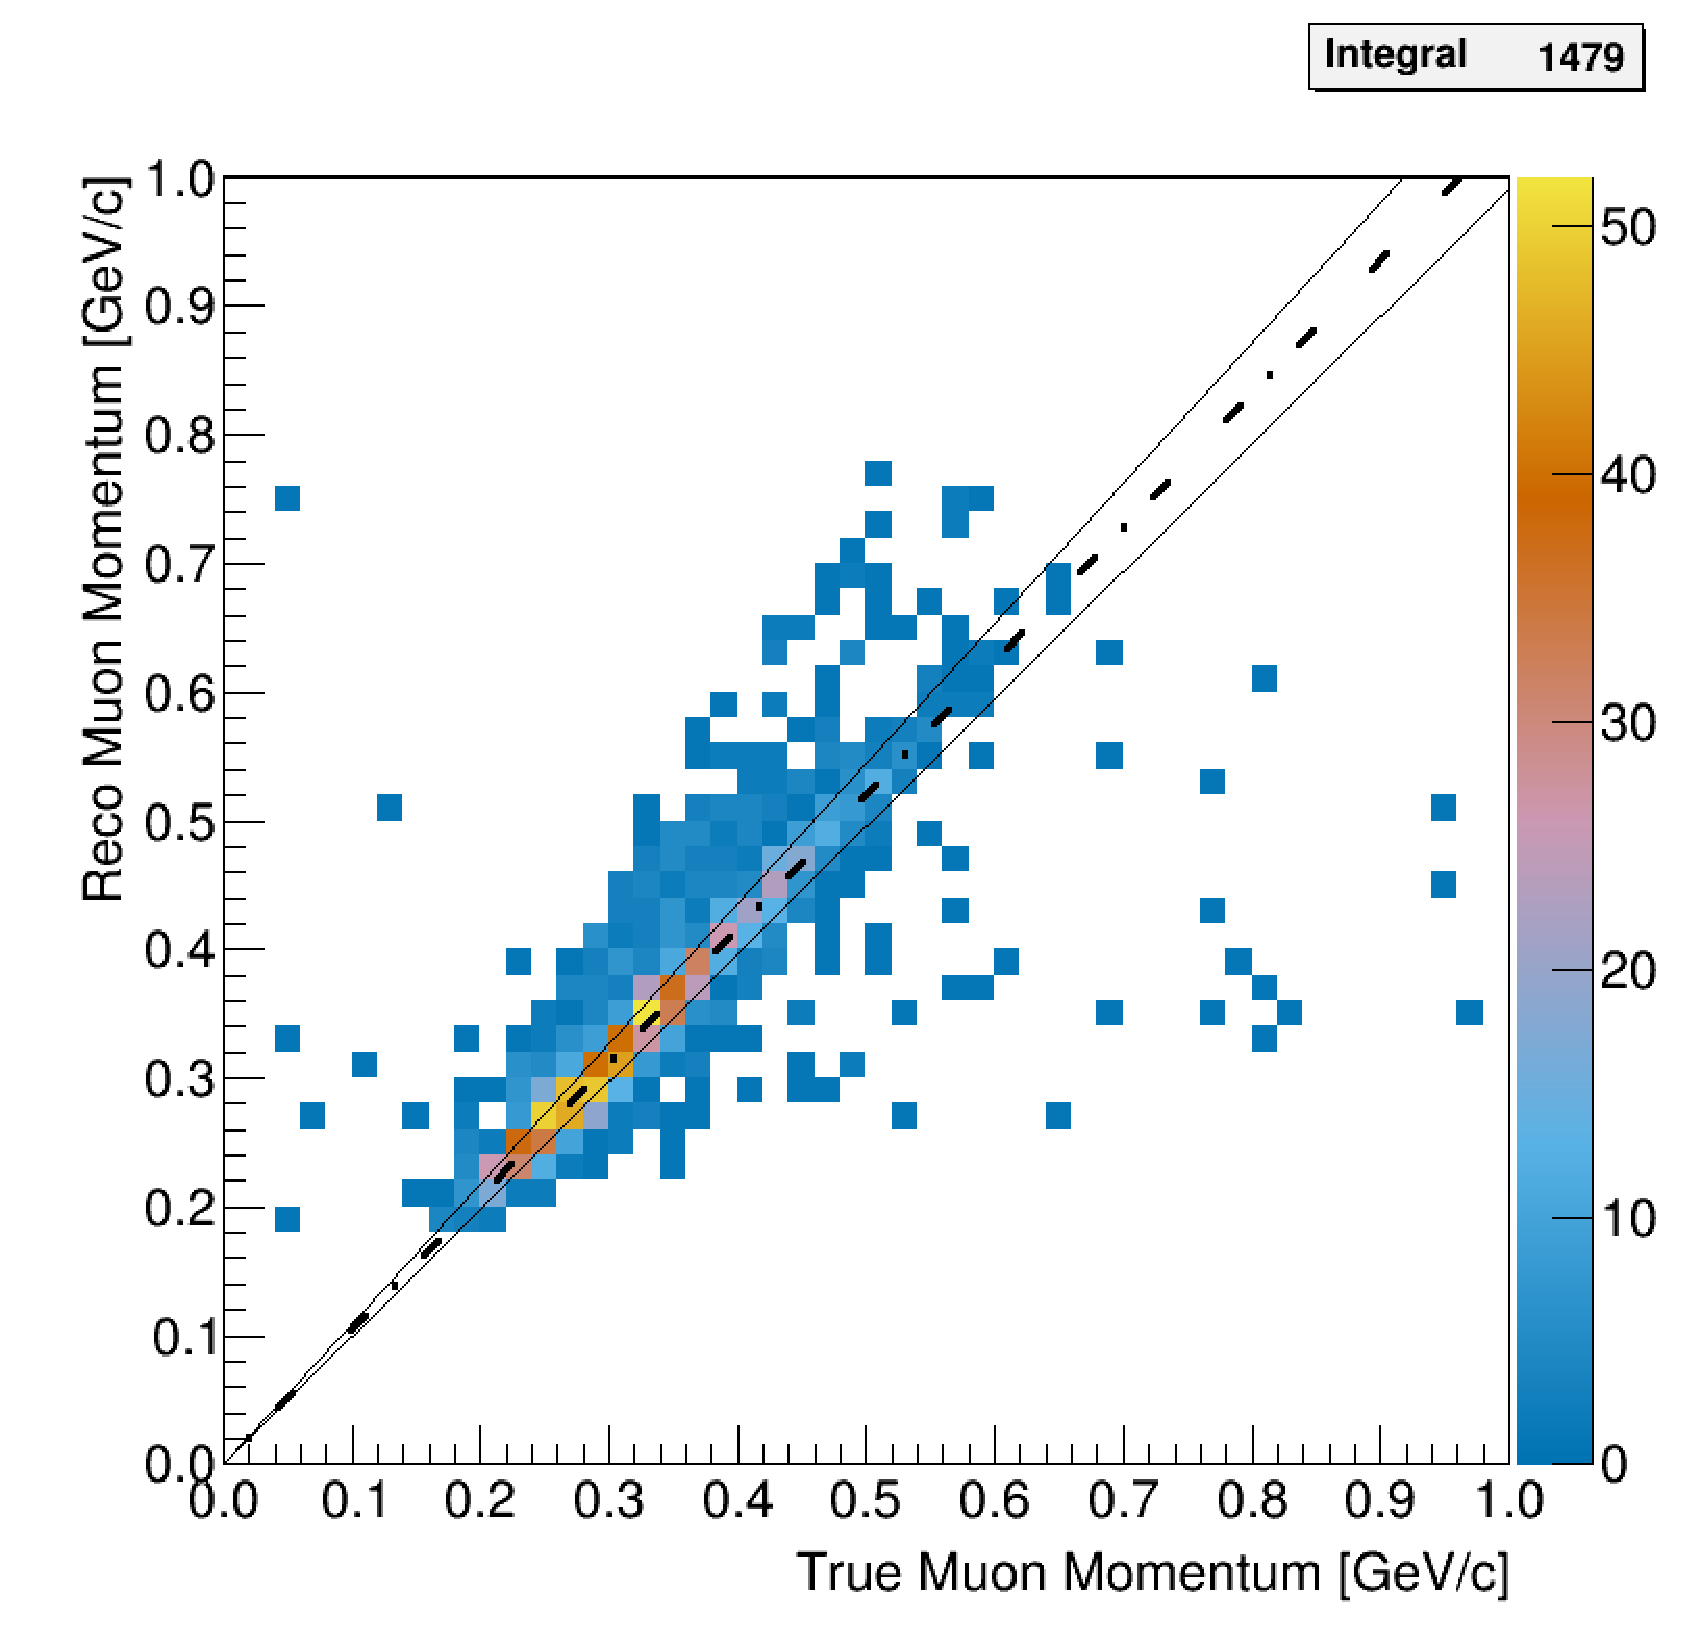
\includegraphics[width=0.48\textwidth]{Figures/P0DCC1pi/Contained_SignalMuons_UnCalib_reco_vs_true_p}
\par\end{centering}
}
\par\end{centering}
\begin{centering}
\subfloat[]{\begin{centering}
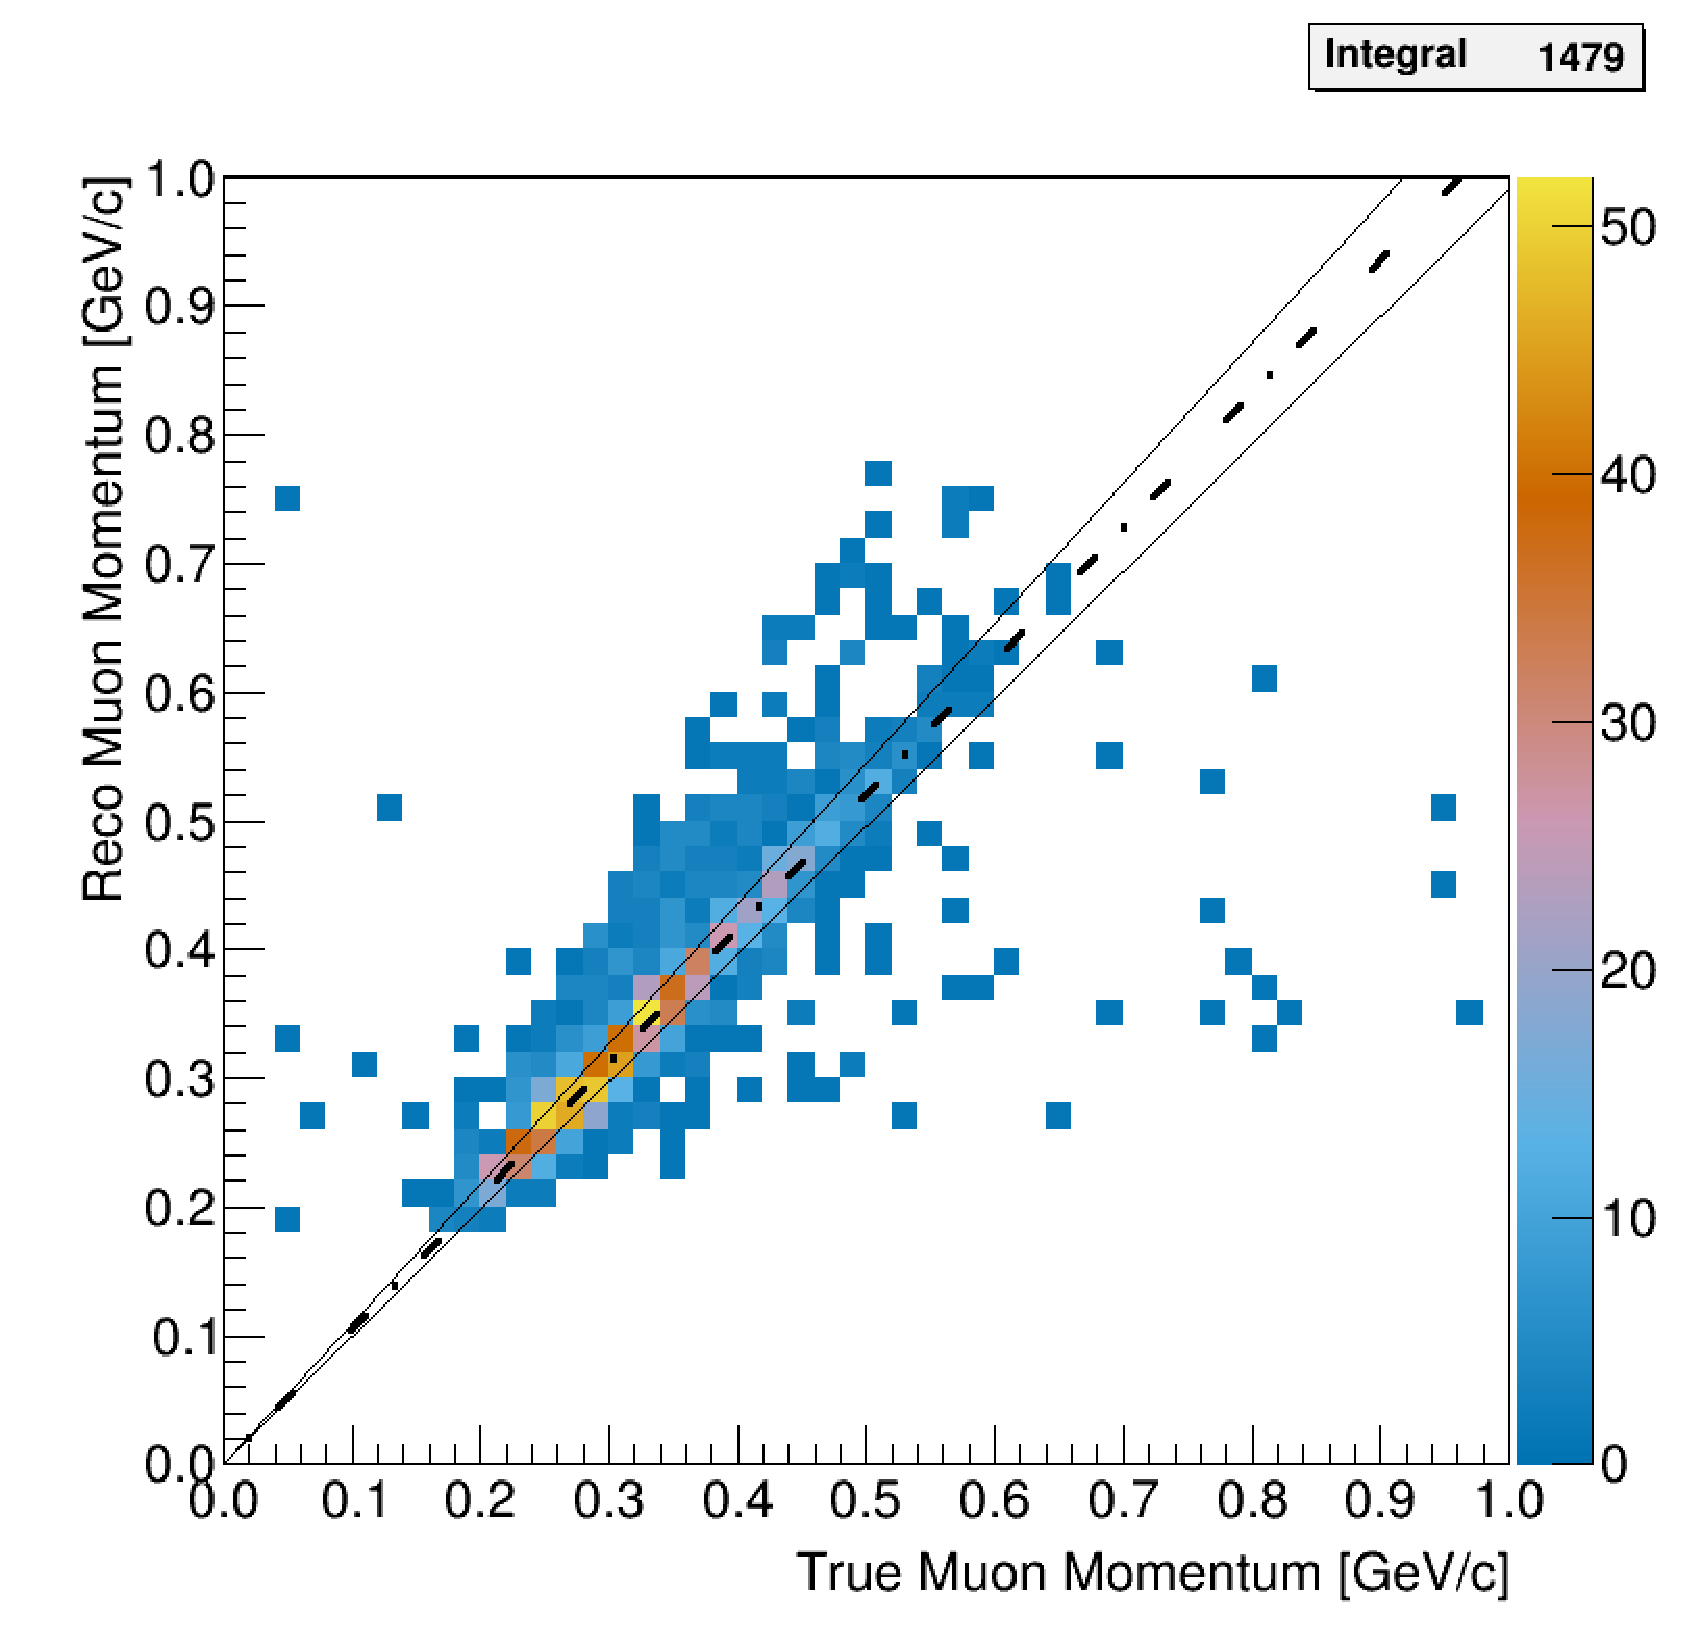
\includegraphics[width=0.48\textwidth]{Figures/P0DCC1pi/Contained_SignalMuons_UnCalib_reco_vs_true_p}
\par\end{centering}
}\subfloat[]{\begin{centering}
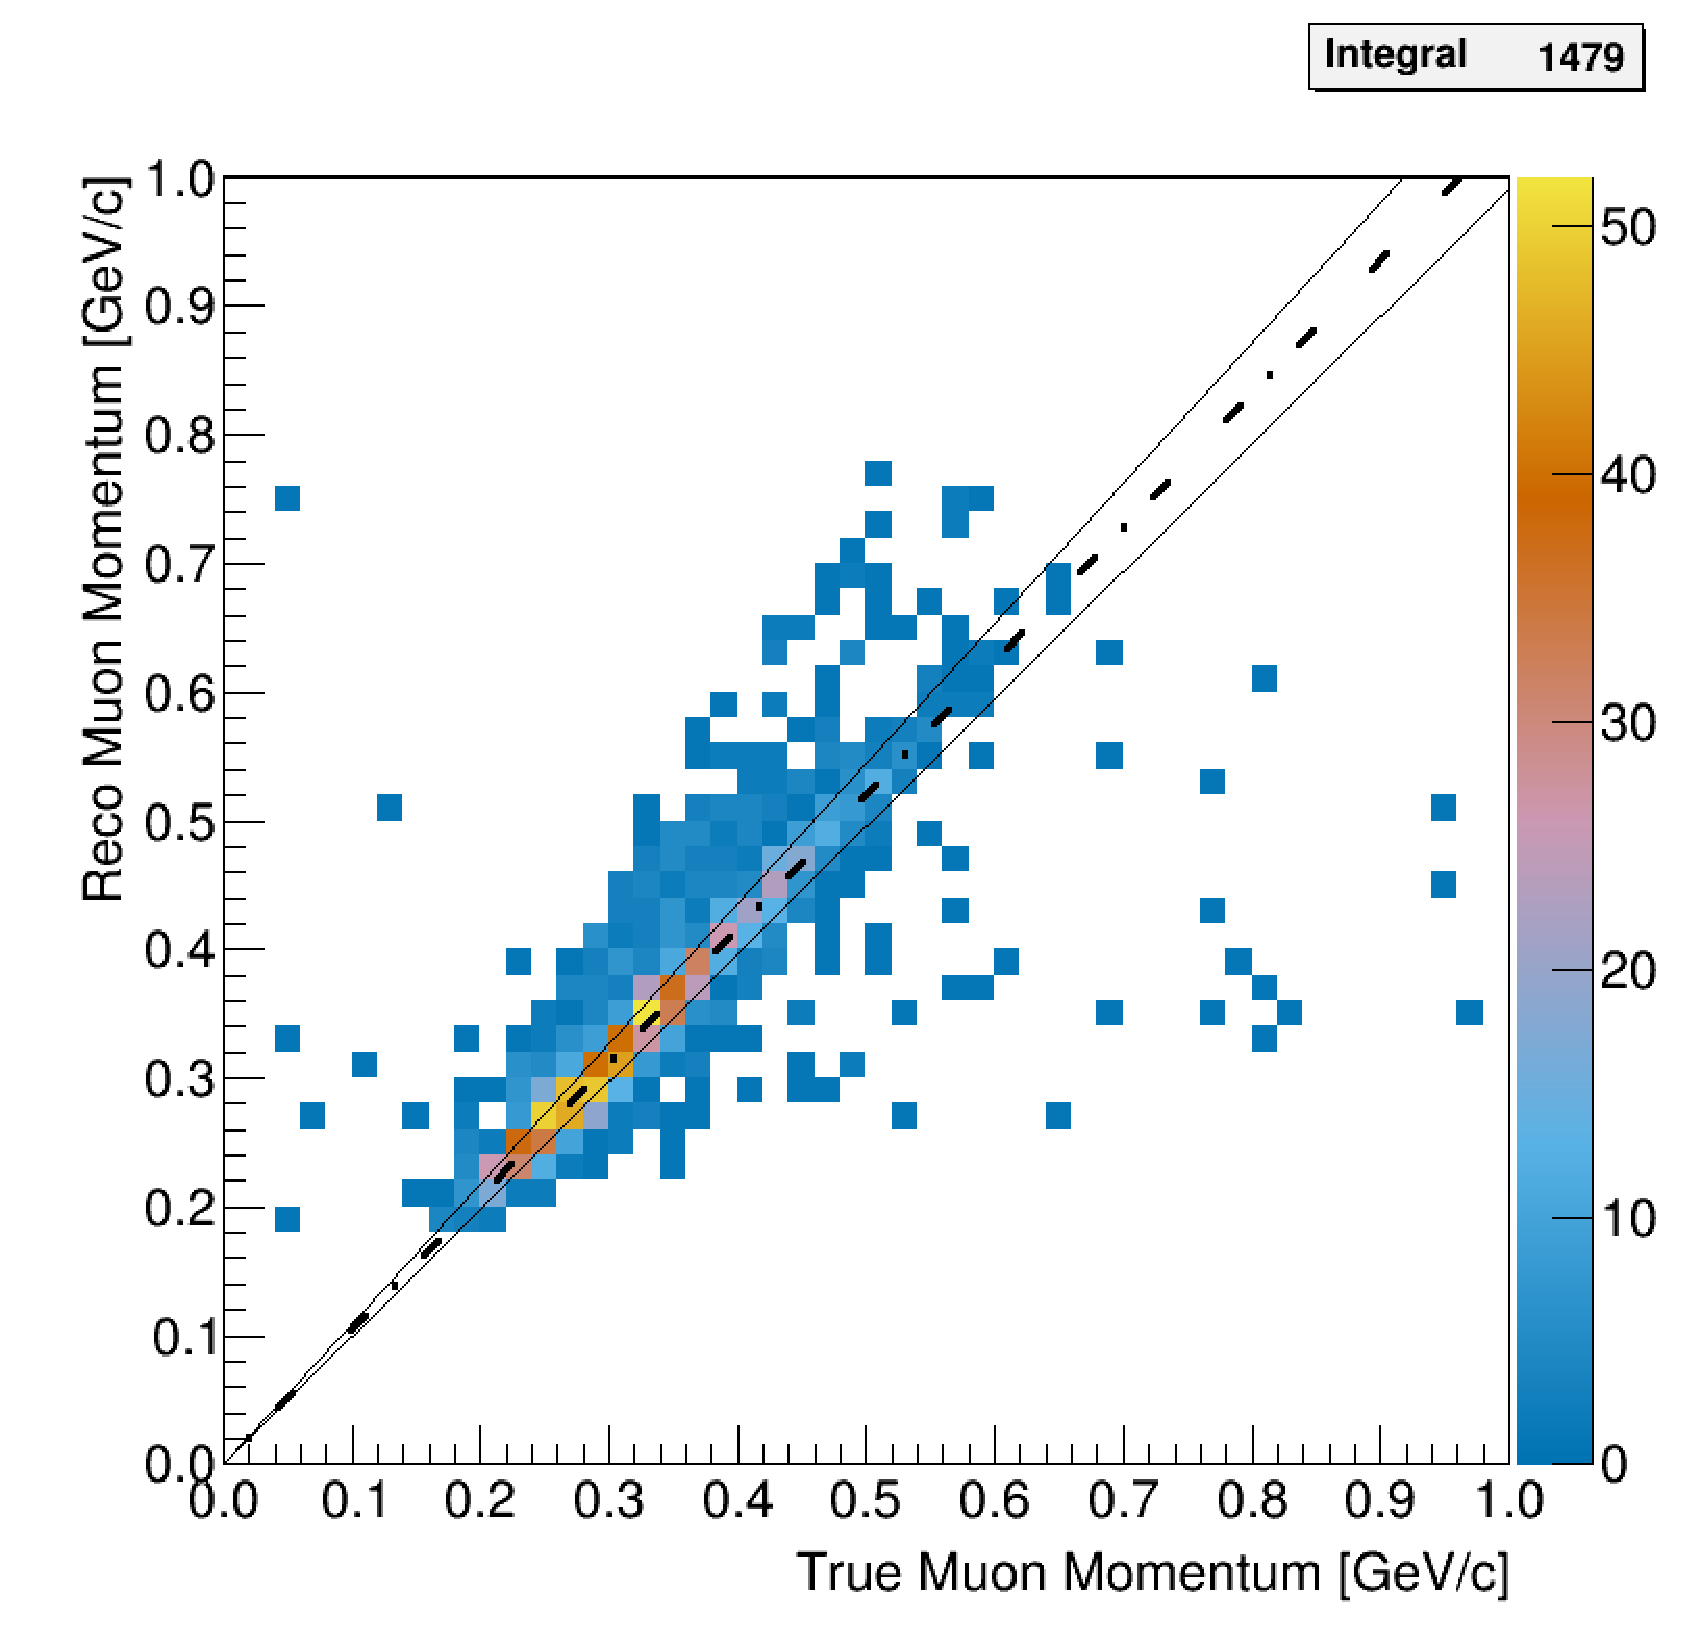
\includegraphics[width=0.48\textwidth]{Figures/P0DCC1pi/Contained_SignalMuons_UnCalib_reco_vs_true_p}
\par\end{centering}
}
\par\end{centering}
\caption{Test}

\end{figure}

\end{document}
